\documentclass[review,times]{elsarticle}

\usepackage[T1]{fontenc}
\usepackage[utf8]{inputenc}
\usepackage{lmodern}
\usepackage[top=4.3cm,bottom=4.8cm,left=4.3cm,right=4.8cm]{geometry}
\usepackage{microtype}
\usepackage{amsmath,amssymb,bm}
\usepackage{graphicx}
\usepackage{booktabs}
\usepackage{tabularx}
\usepackage{array}
\usepackage{float}
\usepackage{caption}
\usepackage{subcaption}
\usepackage{enumitem}
\usepackage{xcolor}
\usepackage{lineno}
\usepackage[hidelinks]{hyperref}
\usepackage[nameinlink,noabbrev]{cleveref}

\graphicspath{{figures/}}
\setlist[itemize]{leftmargin=1.5em,itemsep=0.2em,topsep=0.3em}
\captionsetup{font=footnotesize,labelfont=bf,justification=raggedright,singlelinecheck=false}
\renewcommand{\arraystretch}{1.08}
\newcommand{\method}{PMRC}
\newcommand{\vect}[1]{\mathbf{#1}}
\newcommand{\indicator}{\mathbf{1}}
\newcommand{\eg}{e.g.,\ }
\newcommand{\ie}{i.e.,\ }

\journal{Pattern Recognition}

\begin{document}
\begin{frontmatter}

\title{Post-hoc Prototype-Margin Reliability Calibration for Closed-Set Selective Fine-Grained Recognition under Label Noise}

\author[inst1]{Xianning Zhao\corref{cor1}}
\ead{zhxianning2025@lzu.edu.cn}
\cortext[cor1]{Corresponding author.}

\author[inst1]{Haoyuan Tang}
\author[inst1]{Liang Qiao}

\affiliation[inst1]{
  organization={School of Information Science and Engineering, Lanzhou University},
  city={Lanzhou},
  postcode={730000},
  state={Gansu},
  country={China}
}

\begin{abstract}
\vspace{0.25em}\noindent
Selective classifiers improve reliability by abstaining on uncertain inputs,
but their value depends on how well predictions are ordered before abstention.
We formulate the selective reliability gap after noisy-label training and ask
whether it can be reduced without retraining the classifier. Prototype-margin
reliability calibration (PMRC) constructs class prototypes from observed noisy
labels, combines them with confidence and two-view consistency, and fits a
sample-specific correctness ranker on clean calibration data. It changes only
the acceptance order. In controlled fine-grained experiments, PMRC reduced
AURC by 12.8\% to 19.9\% under high noise, compared with 1.9\% for a clean
control. The improvement held across three training objectives and two
backbones, and transferred to Stanford Dogs with a 28.4\% mean reduction.
WebFG-496 tested conditional activation: the gate selected PMRC on two subsets
and returned to maximum softmax probability (MSP) on the third. PMRC therefore
targets a specific condition: prototype geometry must add correctness
information beyond confidence, and the calibration-side gate decides whether
that condition holds.
\end{abstract}

\begin{keyword}
fine-grained recognition \sep noisy labels \sep selective prediction \sep
calibration
\end{keyword}

\end{frontmatter}

\linenumbers
\pagestyle{plain}

\section{Introduction}

Fine-grained recognition must separate visually similar categories from small, local differences. Part-based and multi-granularity representations have improved this discrimination \citep{lin2015bilinear,du2020pmg}. Web-sourced alternatives reduce annotation cost while introducing closed-set confusion, duplicate images, contextual labels, and open-set noise \citep{wei2022cifar100n,sun2021webfg}.

Noisy-label methods include robust losses and example reweighting \citep{song2023noisysurvey,wang2019sce,ren2018reweight}, sample selection and semi-supervised separation \citep{han2018coteaching,li2020dividemix}, and training-dynamics or disagreement-based strategies \citep{ma2018dimensionality,yu2019disagreement}. These objectives improve the classifier, but they do not directly control which of its predictions remain trustworthy after abstention. For a fixed classifier, the ideal selective rule accepts samples in decreasing order of correctness probability. Its shortfall from that perfect ordering defines a reliability gap that persists even when full-coverage predictions are frozen \citep{geifman2017selective,rabanser2025selectivegap}. In our controlled matrix, the recoverable ordering improvement is 1.9\% on a clean model but 12.8\% to 19.9\% under high label noise. This asymmetry supports treating selective ordering as a target separate from classification accuracy.

Monotone confidence calibration changes probability scale without adding sample-specific evidence. Closing the ordering gap therefore requires a score that can distinguish similarly confident correct and incorrect predictions. \method{} supplies this signal after training: it constructs class prototypes from observed noisy labels, combines prototype margin with confidence and two-view consistency, and fits a correctness ranker on clean calibration data. The classifier and its argmax predictions remain unchanged, so the measured effect is isolated to the acceptance order.

The paper makes three contributions.
\begin{itemize}
  \item a formulation of noisy-label selective reliability as an ordering gap that can be measured while holding full-coverage accuracy fixed;
  \item a classifier-preserving post-hoc procedure that closes part of this gap using observed-label prototype geometry and sample-specific consistency evidence;
  \item a calibration-side applicability diagnostic that selects PMRC when prototype margin carries correctness information and otherwise retains MSP.
\end{itemize}

\section{Background and Related Work}

\subsection{Learning with noisy labels}

Existing approaches include robust losses and adaptive reweighting \citep{wang2019sce,ren2018reweight}, sample selection and semi-supervised separation \citep{han2018coteaching,li2020dividemix}, training-dynamics regularization \citep{ma2018dimensionality,yu2019disagreement}, and label correction \citep{liu2020elr}. Label-error estimation methods further estimate which observed labels are likely incorrect \citep{northcutt2021confident}. \method{} is complementary because it does not alter training data, parameters, or objectives. It targets the order in which a fixed classifier accepts and rejects samples.

\subsection{Selective classification and confidence calibration}

Selective classification ranks samples before choosing a coverage level \citep{geifman2017selective,geifman2019selectivenet,gangrade2021onesided}. Abstention has also been used directly as a device for noisy-label training \citep{thulasidasan2019abstention}. MSP, margin, entropy, energy, temperature scaling, and MaxLogit-pNorm operate directly on classifier outputs \citep{hendrycks2017msp,guo2017calibration,cattelan2024fix}. Calibration metrics and post-hoc methods are reviewed by Silva Filho et al. \citep{silvafilho2023calibration}. k-nearest-neighbor (KNN) agreement and Trust Score use training-feature geometry \citep{jiang2018trust}. A recent decomposition shows that monotone post-hoc calibration can improve probability calibration while leaving much of the selective-classification gap intact \citep{rabanser2025selectivegap}. \method{} also uses feature geometry, but estimates prototypes from observed noisy labels and learns a validation-side correctness ranking.

\subsection{Fine-grained web supervision}

Webly supervised fine-grained recognition combines subtle inter-class differences with imperfect web labels. WebFG-496 provides web-collected training images and clean evaluation images for bird, aircraft, and car subsets \citep{sun2021webfg}. We use this dataset to evaluate selective ordering; top-1 web-classification performance is outside the study.

\subsection{Position of PMRC}

ReCalMatch calibrates pseudo-label reliability during semi-supervised fine-grained training \citep{hong2026recalmatch}. DGCL partitions samples using geometric and semantic consensus during training \citep{guo2027dgcl}. CYFLOD filters or dampens noisy supervision during optimization \citep{gilal2025cyflod}. Evidential methods use Dirichlet evidence to quantify classification uncertainty \citep{sensoy2018evidential}. These methods change training data, objectives, or classifier parameters. \method{} instead operates after training: it freezes the resulting classifier and learns a separate correctness ranking for selective acceptance. This separation makes the algorithm composable with a trained noisy-label pipeline and allows the ranking contribution to be evaluated independently of classification accuracy.

\section{Method}

\begin{figure}[t]
  \centering
  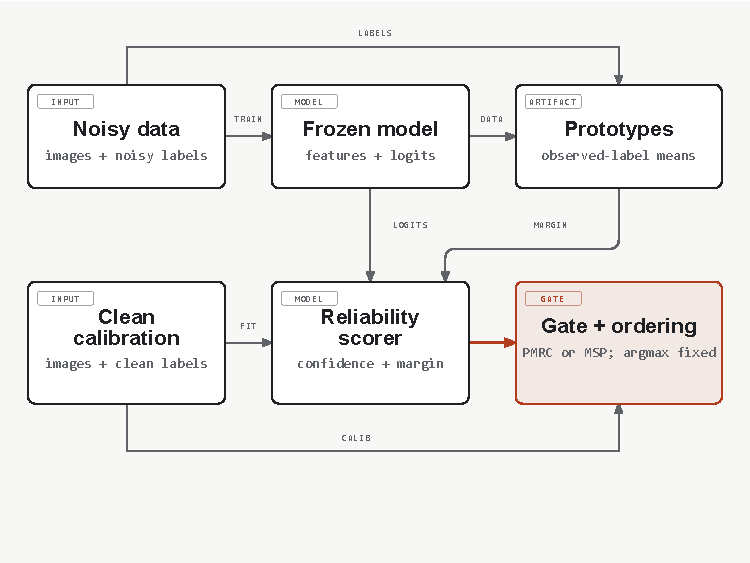
\includegraphics[width=\textwidth]{figureS2_method_overview.pdf}
  \caption{Overview of PMRC. Noisy training labels form class prototypes in the frozen-classifier feature space. A clean calibration set fits a sample-level reliability scorer. At inference, a validation-only gate chooses between PMRC and MSP ordering. The classifier prediction remains unchanged in both branches.}
  \label{fig:method}
\end{figure}

\subsection{The selective reliability gap}

Let a classifier $f_\theta$ be trained on pairs $(\vect{x}_i,\tilde y_i)$, where $\tilde y_i$ may differ from the unknown clean label. Training may use cross-entropy, ELR, or another label-noise method. Before inference, the classifier is frozen. A calibration set $\mathcal{D}_v=\{(\vect{x}_j,y_j)\}_{j=1}^{n_v}$ contains clean labels and is used only to fit a correctness-ranking function.

For a test image $\vect{x}$, the classifier produces
\begin{equation}
  \hat y(\vect{x})=\arg\max_c p_\theta(c\mid\vect{x}).
  \label{eq:prediction}
\end{equation}
\method{} returns a reliability score $r(\vect{x})$ but does not modify $\hat y(\vect{x})$. At coverage $c$, the $c$ fraction of samples with highest reliability is accepted. Since the classifier is frozen, its full-coverage accuracy $a$ is common to all compared scores. Following the selective-classification gap formulation \citep{rabanser2025selectivegap}, a perfect correctness ordering would accept the $c$ fraction of samples with highest correctness probability, giving the selective-accuracy upper bound
\begin{equation}
  a^*(c)=\min\left(1,\frac{a}{c}\right),\qquad c\in(0,1].
  \label{eq:oracle}
\end{equation}
For a reliability score $r$, let $a_r(c)$ be the realized selective accuracy at the same coverage. We study the selective reliability gap
\begin{equation}
  G_r(c)=a^*(c)-a_r(c).
  \label{eq:gap}
\end{equation}
Because $a$ is fixed, comparing two scores on $G_r(c)$ isolates their ranking effect from any change in full-coverage prediction. Throughout the paper, we summarize this ordering difference with empirical AURC. Selective risk is the error rate among accepted samples, and AURC is the area under the resulting risk-coverage curve.

\subsection{Why confidence rescaling leaves a ranking gap}

A single post-hoc transformation of the confidence score cannot introduce sample-specific evidence. Temperature scaling, for example, improves probability calibration, but it does not use class geometry or image-view consistency to separate otherwise similarly confident samples. In the CUB semantic-40 ResNet-50 seed~0 run, temperature scaling changed AURC from 0.2076 to 0.2056, whereas a sample-specific calibration model using prototype and two-view evidence reduced it to 0.1643. The comparison defines the target of PMRC: keep the classifier fixed and add evidence for ordering accepted samples.

\subsection{Noisy-label class prototypes}

Class prototypes are standard feature-space summaries in metric learning \citep{snell2017prototypical}. For every observed class $c$, we normalize each training feature and average the features of samples whose observed label is $c$:
\begin{equation}
  \bm{\mu}_c=
  \frac{\sum_{i:\tilde y_i=c}\vect{z}_i}
  {\left\|\sum_{i:\tilde y_i=c}\vect{z}_i\right\|_2},
  \qquad
  \vect{z}_i=
  \frac{\phi_\theta(\vect{x}_i)}{\|\phi_\theta(\vect{x}_i)\|_2},
  \label{eq:prototype}
\end{equation}
where $\phi_\theta$ denotes the penultimate feature. Clean training labels are not used. If observed labels do not cover a class, PMRC is unavailable for that run and deployment falls back to MSP. Observed-label coverage was complete in every evaluated dataset; exact class counts are reported in the supplement.

We use ``observed-label prototype'' for the deployable construction.
Mechanism tables use ``noisy prototype'' as shorthand for the same quantity;
``clean-oracle prototype'' denotes the non-deployable diagnostic alternative.

For prediction $\hat y$, the prototype margin is
\begin{equation}
  m_{\mathrm{proto}}(\vect{x})=
  \vect{z}^{\top}\bm{\mu}_{\hat y}
  -
  \max_{c\ne\hat y}\vect{z}^{\top}\bm{\mu}_{c}.
  \label{eq:margin}
\end{equation}
This quantity measures whether the feature is more compatible with the predicted class than with its strongest competitor. A second view is computed from a horizontally flipped image and contributes agreement, cosine-similarity, prediction-agreement, and logit-distance descriptors.

\subsection{Reliability calibration}

Ten descriptors are extracted from the frozen model:
\begin{enumerate}[leftmargin=1.6em,itemsep=0.1em,topsep=0.2em]
  \item maximum softmax probability;
  \item top-two probability margin;
  \item negative entropy;
  \item energy;
  \item feature norm;
  \item two-view probability agreement;
  \item two-view feature cosine similarity;
  \item two-view prediction agreement;
  \item logit-view distance;
  \item prototype margin.
\end{enumerate}

On the clean calibration set, the target is
\begin{equation}
  s_j=\indicator\left[\hat y(\vect{x}_j)=y_j\right].
  \label{eq:correctness}
\end{equation}
The descriptors are standardized using calibration statistics, and an L2-regularized logistic model estimates
\begin{equation}
  r(\vect{x})=\sigma\left(\vect{w}^{\top}\psi(\vect{x})+b\right),
  \label{eq:calibrator}
\end{equation}
where $\psi(\vect{x})$ is the standardized descriptor vector. The regularization strength is selected by five-fold cross-validation within the calibration set. Test labels are not used for feature selection, regularization selection, or fitting.

\subsection{Applicability gate}

\method{} is designed to improve ordering when prototype geometry contains information not already represented by MSP. We compute a validation-only diagnostic by dividing calibration samples into five equal-frequency MSP bins and calculating prototype-margin AUROC for correctness within each bin. Let $a_v$ be the sample-weighted AUROC. The deployed score is
\begin{equation}
  \hat r(\vect{x})=
  \begin{cases}
    r(\vect{x}), & a_v>0.5,\\
    \mathrm{MSP}(\vect{x}), & a_v\le0.5.
  \end{cases}
  \label{eq:gate}
\end{equation}
The gate uses clean calibration labels only. It introduces no fitted network parameters, and test labels are not used to choose the score. The threshold of 0.5 denotes no better-than-chance ranking within confidence strata.

\section{Experiments}

\subsection{Datasets and noise protocols}

The primary fine-grained experiments use CUB-200-2011 \citep{wah2011cub}, FGVC-Aircraft \citep{maji2013aircraft}, and Oxford Flowers102 \citep{nilsback2008flowers}. CUB and Aircraft use a 10\% clean calibration split; Flowers102 uses 20\%. The clean test sets contain 5,794, 3,333, and 6,149 images, respectively.

The complete split protocol and sample counts are reported in the Supplementary Material, Evaluation protocols.

Semantic-neighbor noise replaces a requested fraction of training labels using classes selected from the top five nearest pretrained class centroids, weighted by centroid similarity. We distinguish the requested flip rate from the realized observed noise rate, which can differ after class-wise corruption and the exclusion of identity flips. This produces observed rates of 18.5\% and 40.7\% for requested CUB rates of 20\% and 40\%, 20.1\% and 40.2\% for Aircraft, and 25.0\% and 37.5\% for the two Flowers102 requests. CUB symmetric noise reaches 40.7\%. A clean CUB model is used as the control.

CIFAR-100N supplies real human annotation noise \citep{wei2022cifar100n}. A class-stratified 2\% split of the official training set forms a 1,000-image clean calibration set, leaving 49,000 noisy training images and 10,000 clean test images. The measured noise rate is 40.2\%.

WebFG-496 provides real webly supervised fine-grained data \citep{sun2021webfg}. Its bird, aircraft, and car subsets contain 18,388, 13,503, and 21,448 training images with 200, 100, and 196 classes. The official clean validation images were split once into 10\% calibration and 90\% test data, producing 584/5,210, 300/3,033, and 783/7,258 calibration/test images. All classifier seeds shared the same partition. Aircraft and car use three seeds. The initial three Bird seeds were heterogeneous and all triggered MSP fallback, so we registered three additional seeds before inspecting their results to test whether this fallback regime was reproducible. Bird therefore uses six seeds: the initial runs and a preregistered replication with seeds 3--5. The replication protocol fixed the split, classifier configuration, epoch count, gate threshold, evaluation metrics, and the requirement to report all three added seeds without replacement.

Stanford Dogs provides an independent 120-class fine-grained downstream dataset \citep{khosla2011dogs}. We preserved the official train/test membership and removed 120 train-side images whose exact pixel hashes occurred in test or more than once in train. Exactly five retained train images per class formed a 600-image clean validation/calibration split, leaving 13,686 noisy training images; the 6,174 official test images remained untouched. The gate threshold and all split rules were frozen before training.

\subsection{Classifiers and implementation}

The fixed matrix uses ImageNet-pretrained ResNet-50 classifiers trained with ELR. CUB and Aircraft use 20 epochs; Flowers102 uses 40. ELR uses $\beta=0.9$ and $\lambda=3.0$. Two additional CUB models use cross-entropy under semantic and symmetric 40\% noise. Three matched CUB semantic-40 models use GCE with $q=0.7$ \citep{zhang2018gce}. CIFAR-100N uses an ImageNet-pretrained ResNet-18 at $64\times64$, batch size 256, learning rate $2\times10^{-4}$, and eight ELR epochs. Three CUB semantic-40 ResNet-18 runs (seeds 0--2) test backbone dependence. WebFG uses ImageNet-pretrained ResNet-50 classifiers with the first stage frozen, $224\times224$ inputs, batch size 64, learning rate $10^{-4}$, and 12 ELR epochs.

All main ELR settings use three seeds, with six for the WebFG bird replication. The 42 primary evaluations comprise 30 controlled classifiers and 12 WebFG classifiers; the controlled total includes the clean CUB control and two additional single-seed cross-entropy models. Five additional training-objective runs, comprising two CE seeds and three GCE seeds, are analyzed separately. Three Stanford Dogs ResNet-50 classifiers test downstream dataset and split transfer under 40\% semantic-neighbor noise. Paired bootstrap confidence intervals compare AURC for \method{} and MSP by resampling identical test images; the interval captures test-sampling uncertainty conditional on each trained model, rather than uncertainty over training seeds. On the RTX 5060 Laptop GPU, a complete controlled post-hoc analysis took 59 to 93 seconds, and two-view descriptor extraction cost 1.74 to 2.57 times one ordinary classifier forward pass. Five-fold calibration over four L2 candidates took 4.7 to 6.5 seconds. WebFG post-hoc analysis took approximately 5 to 10 minutes per subset after training.

To avoid mixing inferential units, we distinguish five scopes: the 42-run primary closed-set evaluation, five additional training-objective runs, secondary reanalyses of frozen models, three separately trained CUB open-set classifiers, and three Stanford Dogs downstream test classifiers. The nine-run training-objective comparison reuses four primary runs and adds these five runs. Unless stated otherwise, gate and risk counts refer only to the 42-run primary evaluation.

\subsection{Q1: How large is the selective reliability gap under label noise?}

\paragraph{Setup.} Q1 tests whether noisy-label training changes the acceptance ordering after full-coverage accuracy is fixed. We begin with the controlled matrix, then vary the training objective, dataset domain, human-label source, and evaluation conditions.

\subsubsection{Controlled fine-grained matrix}

\Cref{fig:controlled} summarizes the controlled evidence, and \Cref{tab:controlled} reports the corresponding numeric results. In CUB semantic-40 ResNet-50 experiments, mean AURC decreased from 0.2109 to 0.1769, a 16.2\% relative reduction. Corresponding reductions were 17.5\% for CUB symmetric-40, 12.8\% for Aircraft semantic-40, and 19.9\% for Flowers102 semantic-37.5. All seed-level paired intervals in these primary settings were below zero.

Lower-noise settings also showed consistent gains: 7.0\% on CUB semantic-20, 13.8\% on Aircraft semantic-20, and 13.4\% on Flowers102 semantic-25. The clean CUB control changed from AURC 0.0456 to 0.0447, a 1.9\% change whose interval crossed zero. This contrast is consistent with addressing a noise-induced reliability gap rather than applying a uniformly beneficial confidence transform.

At 90\% coverage, mean risk decreased from 0.3736 to 0.3660 on CUB semantic-40, from 0.3331 to 0.3236 on CUB symmetric-40, from 0.4117 to 0.4033 on Aircraft semantic-40, and from 0.3008 to 0.2904 on Flowers102 semantic-37.5.

\begin{figure}[t]
  \centering
  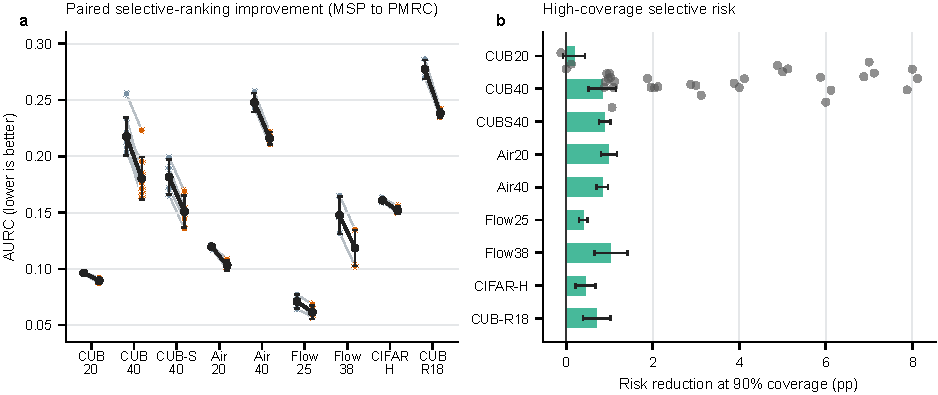
\includegraphics[width=\textwidth]{figure1_pmrc_effect.pdf}
  \caption{\method{} improves selective ranking under controlled label noise. (a) Paired test AURC for MSP and \method{} across seeds and settings. Thin lines connect the same seed; black segments show means. (b) Reduction in selective risk at 90\% coverage. Dots show individual seeds and bars show seed means.}
  \label{fig:controlled}
\end{figure}

\begin{table}[t]
\centering
\caption{Controlled test-set results. Lower AURC is better. Improvement is
reported as mean $\pm$ standard deviation over training seeds of per-seed
relative AURC reductions; this SD is not a test-image uncertainty estimate.
The parentheses report backbone/objective and seed count. R50 and R18 denote
ResNet-50 and ResNet-18; sem and sym denote semantic-neighbor and symmetric
noise. The two single-seed CE rows belong to the primary matrix; the separate
three-seed CE/ELR/GCE comparison is reported in the supplement.}
\label{tab:controlled}
\fontsize{10}{12}\selectfont
\setlength{\tabcolsep}{4pt}
\begin{tabularx}{\textwidth}{@{}>{\raggedright\arraybackslash}Xrrr@{}}
\toprule
Setting & MSP AURC & \method{} AURC & \shortstack{Improvement\\(mean $\pm$ SD)} \\
\midrule
CUB sem-20 (R50/ELR, 3) & 0.0963 & 0.0895 & 7.0 $\pm$ 2.0\% \\
CUB sem-40 (R50/ELR, 3) & 0.2109 & 0.1769 & 16.2 $\pm$ 4.6\% \\
CUB sym-40 (R50/ELR, 3) & 0.1755 & 0.1448 & 17.5 $\pm$ 1.6\% \\
Aircraft sem-20 (R50/ELR, 3) & 0.1195 & 0.1031 & 13.8 $\pm$ 3.2\% \\
Aircraft sem-40 (R50/ELR, 3) & 0.2476 & 0.2159 & 12.8 $\pm$ 1.4\% \\
Flowers sem-25 (R50/ELR, 3) & 0.0710 & 0.0615 & 13.4 $\pm$ 3.7\% \\
Flowers sem-37.5 (R50/ELR, 3) & 0.1475 & 0.1184 & 19.9 $\pm$ 2.1\% \\
CIFAR-100N human (R18/ELR, 3) & 0.1609 & 0.1519 & 5.6 $\pm$ 1.0\% \\
CUB sem-40 (R18/ELR, 3) & 0.2771 & 0.2380 & 14.1 $\pm$ 1.2\% \\
CUB sem-40 (R50/CE, 1) & 0.2090 & 0.1664 & 20.4\% \\
CUB sym-40 (R50/CE, 1) & 0.1990 & 0.1689 & 15.1\% \\
CUB clean (R50/ELR, 1) & 0.0456 & 0.0447 & 1.9\% \\
\bottomrule
\end{tabularx}
\end{table}

\subsubsection{Training-objective transfer}

We evaluated CE, ELR, and GCE on CUB semantic-40 for three seeds each while holding the architecture, data splits, prototype construction, and post-hoc protocol fixed. All nine runs improved, with all nine paired test-image bootstrap intervals below zero. Mean AURC reductions were 18.0\% for CE (0.2327 to 0.1914), 16.2\% for ELR (0.2109 to 0.1769), and 17.5\% for GCE (0.2090 to 0.1725); the corresponding seed standard deviations were 4.6, 4.6, and 1.5 percentage points. PMRC also had lower AURC than temperature scaling, pNorm, KNN, and Trust Score in every one of the nine runs (Supplementary Material, Training-objective transfer).

\subsubsection{Independent downstream dataset and split transfer}

We then evaluated the protocol-fixed procedure on Stanford Dogs, a 120-class dataset that did not contribute to method design. The official test split was untouched, and exactly five retained official-train images per class formed the 600-image clean validation/calibration partition after exact train-side duplicate removal. With 40\% semantic-neighbor noise over 13,686 training images, mean AURC decreased from 0.0852 to 0.0610, a 28.4\% relative reduction (seed standard deviation 1.8\%). Seed-wise reductions were 28.6\%, 26.5\%, and 30.1\%, and every paired bootstrap interval was below zero. Mean risk at 90\% coverage decreased from 0.1858 to 0.1650. The unchanged gate selected PMRC in all three runs, with validation AUROC values of 0.853, 0.785, and 0.816. Gated PMRC therefore equalled direct PMRC and improved on MSP in every seed. PMRC also had lower AURC than temperature scaling, pNorm, KNN, and Trust Score in every seed; their mean values were 0.0801, 0.0809, 0.0743, and 0.1237, respectively. Because Stanford Dogs is derived from ImageNet, the result establishes downstream dataset and split transfer under a fixed protocol; a pretraining-independent real-web label domain is outside this test. Seed-level results are reported in the Supplementary Material, Independent downstream dataset and split transfer.

\subsubsection{Real human noise and backbone transfer}

On CIFAR-100N, \method{} reduced AURC from 0.1609 to 0.1519, a 5.6\% relative improvement. The reductions across three seeds were 6.4\%, 5.9\%, and 4.5\%, all with confidence intervals below zero. The compact $64\times64$ ResNet-18 protocol adds real human annotation noise and a second resolution regime, while the ResNet-50 matrix provides the architecture-matched comparison. Under CUB semantic-40 with ResNet-18, mean AURC decreased from 0.2771 to 0.2380 across seeds 0--2, a 14.1\% relative improvement. Seed-level reductions were 13.9\%, 13.0\%, and 15.4\%, again with confidence intervals below zero. These runs show that the controlled fine-grained conclusion extends across the original ResNet-50 and synthetic-noise experiments.

\paragraph{Takeaway.} PMRC reduces the ranking gap across the tested noise, training objectives, backbones, and downstream data while full-coverage predictions remain fixed.

\subsection{Q2: Does prototype geometry carry information beyond confidence?}

\paragraph{Setup.} Q2 asks whether the gain reflects information in class geometry rather than a monotone confidence transform. We compare four selective scoring families and isolate the contribution and behavior of the prototype margin.

\subsubsection{Selective-baseline comparison}

Temperature scaling, MaxLogit-pNorm, KNN label agreement, and Trust Score were evaluated on all 30 controlled models. \Cref{tab:baselines} summarizes the comparisons. \method{} achieved lower AURC than KNN in 29 of 30 comparisons, pNorm in 29 of 30, and Temperature scaling and Trust Score in all 30. The two remaining comparisons were near ties: KNN on CUB symmetric-40 with cross-entropy (0.1681 versus 0.1689) and pNorm on the clean CUB control (0.0435 versus 0.0447). All baselines share the same calibration and test splits. Temperature scaling, pNorm, KNN, and Trust Score select their respective hyperparameters on calibration data only.

WebFG shows why the gate is needed. PMRC has lower AURC than temperature scaling in 9 of 12 runs, pNorm in 5 of 12, KNN agreement in 9 of 12, and Trust Score in 4 of 12. Baseline rankings track the two regimes: KNN and Trust Score remain competitive in Bird, whereas PMRC is favored in Aircraft and Car. Q3 tests whether a calibration-side diagnostic can separate these regimes.

\begin{table}[t]
\centering
\caption{Selective-baseline summary. Entries report mean AURC (PMRC wins / available runs). Lower is better.}
\label{tab:baselines}
\fontsize{10}{12}\selectfont
\begin{tabularx}{\textwidth}{@{}>{\raggedright\arraybackslash}p{2.7cm}*{4}{>{\centering\arraybackslash}X}@{}}
\toprule
Evaluation set & Temperature & pNorm & KNN & Trust \\
\midrule
Controlled (30) & 0.1622 (30/30) & 0.1590 (29/30) & 0.1632 (29/30) & 0.1823 (30/30) \\
WebFG (12) & 0.0889 (9/12) & 0.0877 (5/12) & 0.0933 (9/12) & 0.0859 (4/12) \\
\bottomrule
\end{tabularx}
\end{table}

\begin{figure}[t]
  \centering
  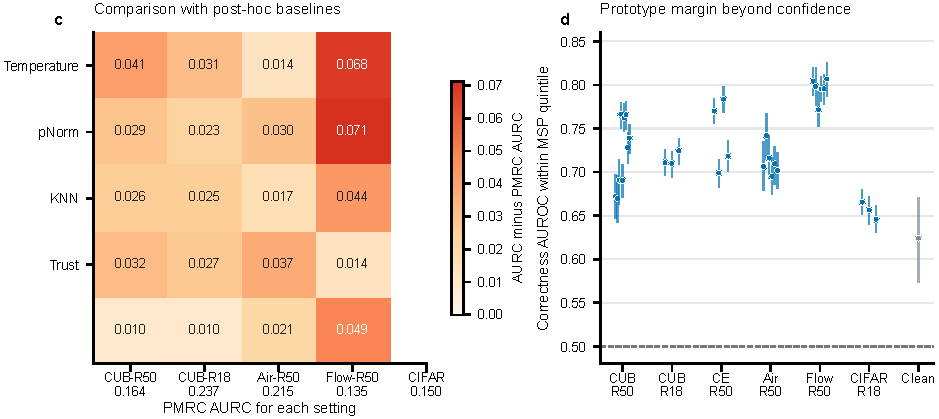
\includegraphics[width=\textwidth]{figure1_pmrc_mechanism.pdf}
  \caption{Evidence that the PMRC gain is not a monotone confidence transform. (a) Difference between each selective baseline's AURC and PMRC AURC for representative models. Positive values indicate worse AURC than PMRC. (b) Correctness AUROC of prototype margin within equal-frequency MSP quintiles; dots are runs and vertical lines are paired bootstrap 95\% intervals. The dashed line marks chance.}
  \label{fig:mechanism}
\end{figure}

\subsubsection{Prototype-information diagnostics}

To test whether prototype margin only re-expresses MSP, samples were partitioned into five equal-frequency MSP strata and prototype margin was used to rank correctness within each stratum. Across the 30 controlled models, the weighted within-stratum AUROC remained above 0.5. WebFG supplied the opposite boundary: all six bird values were below 0.5, while all aircraft and car values exceeded 0.59.

In the corresponding feature-group ablation, adding the prototype-margin group to the confidence-plus-two-view model reduced mean AURC from 0.2081 to 0.1778 on CUB semantic-40, from 0.1595 to 0.1552 on CIFAR-100N, from 0.1235 to 0.1198 on WebFG aircraft, from 0.0836 to 0.0778 on WebFG car, and from 0.0794 to 0.0773 across bird seeds.

The prototype-source ablation evaluated five representative runs. Observed-label prototypes outperform no-prototype and shuffled-prototype controls in all five runs, and outperform ImageNet-feature prototypes in three of five runs. On Flowers102, ImageNet-feature prototypes achieve lower AURC (0.1292 versus 0.1347), and both prototype variants beat the no-prototype control. The results point to geometry quality as a condition for the gain without favoring one prototype source across all datasets. Clean-label oracle prototypes remain a stronger diagnostic upper bound.

We further compared clean-oracle and observed-label prototypes on eight representative runs (Supplementary Material, Prototype contamination and concentration). Their mean cosine similarity is 0.977 to 0.994 on CUB, Aircraft, and CIFAR-100N and 0.941 to 0.952 on Flowers102. Corrupted training samples systematically have smaller margins to their observed-label prototypes, with corruption-ranking AUROC between 0.766 and 0.937 across all eight runs. A class-level median split then tests whether gains track feature geometry and prototype fidelity (Supplementary Material, Class-level prototype factor partition). PMRC gains are larger in high-concentration classes (22.8\% versus 11.3\%; paired low-minus-high difference -11.5 percentage points, 95\% CI -19.7 to -4.4) and in high-fidelity classes (20.8\% versus 11.4\%; difference -9.4 points, CI -13.9 to -5.5), with all 8/8 runs favoring the high groups. These diagnostics localize the useful signal in class geometry and prototype fidelity. Clean prototypes serve as a diagnostic upper bound.

A second intervention changes only the samples used to construct prototypes while holding the classifier and test set fixed. All-noisy prototypes produce a mean relative PMRC gain of 15.7\%. Filtering the highest-loss 40\% of samples within each observed class raises this to 16.9\%, a gain of 1.18 points over all-noisy prototypes (95\% CI 0.72 to 1.68; 8/8 runs). Clean-oracle prototypes reach 31.7\%, adding a further 14.77 points over the deployable filter (CI 11.18 to 18.44; 8/8 runs). The large oracle headroom shows that prototype contamination discards usable information, while the smaller loss-filter gain locates additional headroom in prototype purification.

\paragraph{Takeaway.} Prototype margin carries correctness information beyond MSP in some classes but not others. The applicability gate uses this condition to decide between PMRC and MSP ordering.

\subsection{Q3: When should PMRC be activated, and where does it stop?}

\paragraph{Setup.} Q3 tests the applicability gate on real web supervision and under operational risk and closed-set boundary conditions. The gate uses clean calibration data only and retains a fixed decision threshold.

\subsubsection{WebFG gate behavior}

WebFG identifies two operating regimes for the same post-hoc procedure (\Cref{fig:webfg}). Aircraft and car used three seeds each. Bird used six to test reproducibility of the fallback decision after the initial three seeds were heterogeneous and all selected MSP. \Cref{tab:webfg} reports the subset means; seed-wise ranges are reported in the Supplementary Material. Positive change denotes relative AURC reduction.

\begin{table}[t]
\centering
\caption{WebFG-496 results and applicability-gate decisions. Bird includes three initial and three preregistered replication seeds; the replication tests whether the fallback regime observed in the initial heterogeneous seeds reproduces. The within-MSP AUROC column reports held-out test values; gate selection uses the corresponding calibration values.}
\label{tab:webfg}
\fontsize{10}{12}\selectfont
\setlength{\tabcolsep}{4pt}
\begin{tabular}{@{}lrrrr@{}}
\toprule
Subset & MSP AURC & \method{} AURC & Mean change & Gate \\
\midrule
Bird (6 seeds) & 0.0773 & 0.0777 & -0.51\% & 0/6 \\
Aircraft (3 seeds) & 0.1203 & 0.1170 & +2.83\% & 3/3 \\
Car (3 seeds) & 0.0794 & 0.0768 & +3.24\% & 3/3 \\
\bottomrule
\end{tabular}
\end{table}

Exact seed-level AURC values and paired bootstrap intervals for WebFG are reported in the Supplementary Material, WebFG seed-level results.

The Bird subset defines the fallback regime. Direct PMRC lies 0.51\% below MSP in mean AURC; five of six seeds do not improve, and seed~3 has a paired interval below zero. Aircraft and Car move in the opposite direction, with two of three paired intervals below zero in each subset. Mean risk at 90\% coverage decreases from 0.1901 to 0.1873 for Bird, from 0.2653 to 0.2635 for Aircraft, and from 0.1929 to 0.1885 for Car.

The calibration diagnostic separates the two regimes. On test data, all six Bird within-MSP prototype AUROC values range from 0.434 to 0.477, while Aircraft and Car range from 0.592 to 0.647. On calibration data, which is what the gate observes, Bird ranges from 0.363 to 0.488, Aircraft from 0.592 to 0.703, and Car from 0.677 to 0.706. At the fixed threshold of 0.5, the gate reverts to MSP for all Bird seeds and retains \method{} for all Aircraft and Car seeds.

Across all 42 evaluations with complete calibration caches, the gate selects \method{} in 36 runs and MSP in the six Bird runs. Test AURC improves relative to MSP in all 36 selected cases; by construction, the six fallback cases equal MSP. Test outcomes do not enter the decision.

A threshold sweep from 0.45 to 0.60 retained zero regressions across the original test splits, with mean AURC gains between 9.8\% and 10.0\%. Across class-disjoint evaluations, the non-regression rate increased from 87.8\% at 0.45 to 92.2\% at 0.60, while mean gated gains remained between 8.3\% and 8.4\%. The selected threshold of 0.5 therefore lies in a broad stable interval rather than on a single favorable cutoff.

We also test within-family transfer by selecting the gate threshold from two WebFG subsets and applying it to the third (Supplementary Material, Gate transfer and lower-bound checks). Candidate thresholds come from a fixed $0.30$--$0.80$ grid and are selected independently in each fold using source-subset validation outcomes only. The three folds select thresholds 0.42, 0.50, and 0.42, retain PMRC for all held-out Aircraft and Car seeds with mean test gains of 2.8\% and 3.2\%, and fall back for all six held-out Bird seeds. A stricter rule based on the fifth percentile of 500 calibration AUROC bootstrap resamples makes the same 36 selections. The Stanford Dogs experiment provides the independent downstream test; this WebFG analysis measures transfer within the same data family.

\begin{figure}[t]
  \centering
  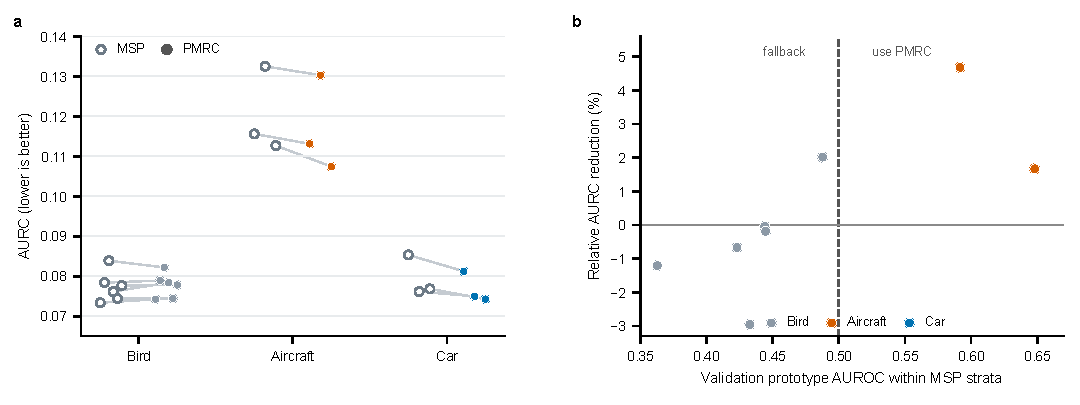
\includegraphics[width=\textwidth]{figure2_webfg_gate.pdf}
  \caption{A calibration-only prototype-signal gate explains the heterogeneous WebFG result. This WebFG-specific analysis complements the controlled within-MSP analysis in \Cref{fig:mechanism}(b). (a) Test AURC of MSP and \method{} for bird, aircraft, and car. Aircraft and car contain three classifiers; bird contains six, comprising three initial and three preregistered replication seeds. The additional bird seeds were registered after the initial three-seed result was heterogeneous and all three selected MSP, so the replication tests fallback reproducibility rather than selecting a favorable seed. All subsets share one fixed clean calibration/test partition. Filled points are \method{} and open points are MSP. (b) Relative test AURC reduction as a function of calibration within-MSP prototype AUROC. The dashed line is the fixed 0.5 gate threshold. All six bird seeds fall below the threshold and return to MSP; all aircraft and car seeds exceed it and retain \method{}. AUROC is computed on the clean calibration split without test labels.}
  \label{fig:webfg}
\end{figure}

\subsubsection{Decision cost and risk-controlled coverage}

We converted score ordering into an acceptance rule with thresholds selected on clean calibration data (\Cref{tab:risk}). At 5\%, 10\%, and 15\% target risks, PMRC increases test coverage in 36, 38, and 37 of 42 runs, with mean gains of 7.7, 8.3, and 7.5 percentage points. Improved ordering and finite-sample risk control are distinct objectives, so we report realized target violations alongside coverage. At the three targets, these occur in 26/42, 25/42, and 27/42 PMRC runs, compared with 24/42, 21/42, and 19/42 MSP runs. Paired McNemar tests show no difference at 5\% ($p=0.804$) or 10\% ($p=0.424$); at 15\%, PMRC has more violations (10 PMRC-only versus 2 MSP-only, $p=0.039$) over the fixed run set. The ordering gain therefore calls for an explicit finite-sample controller when certification is required.

\begin{table}[t]
\centering
\caption{Risk-constrained acceptance over 42 evaluations. Thresholds are selected on clean calibration data and evaluated on fixed test splits. The final two columns count realized test risks above the target; these are empirical outcomes, not guarantees. pp denotes percentage points and viol. denotes violations.}
\label{tab:risk}
\fontsize{10}{12}\selectfont
\setlength{\tabcolsep}{4pt}
\begin{tabular}{@{}rrrrr@{}}
\toprule
Target & Higher \method{} coverage & Mean gain & MSP viol. & \method{} viol. \\
\midrule
5\% & 36/42 & +7.7 pp & 24/42 & 26/42 \\
10\% & 38/42 & +8.3 pp & 21/42 & 25/42 \\
15\% & 37/42 & +7.5 pp & 19/42 & 27/42 \\
\bottomrule
\end{tabular}
\end{table}

Decision-cost analysis identifies the same practical direction: PMRC has lower mean test cost in 38/42 runs when rejection cost is 0.25 or 0.50, and at 0.50 the mean cost decreases from 0.2886 to 0.2740. With a split Learn-then-Test controller \citep{angelopoulos2025ltt,angelopoulos2024conformal}, PMRC accepts more samples than MSP at 10\% and 15\% target risks under the same Clopper--Pearson family-wise bound, with no accepted-run risk violation at either target. The 5\% target is reported in the supplement because the finite-sample procedure accepts few samples at that operating point. Complete empirical-risk, Learn-then-Test, and decision-cost results are in the Supplementary Material.

\subsubsection{Robustness and the closed-set boundary}

The main experiments use a clean, class-covering calibration set. Frozen-feature stress tests show that gated PMRC retains a mean relative AURC gain of 6.7\% with 20\% calibration-label corruption and 7.6\% with 50\% of calibration classes missing. When 20\% or 40\% of classes are excluded from calibration, mean gated gains on the held-out classes are 8.5\% and 8.4\%. These results support operation when the calibration set is not perfectly clean or class-complete. Full results appear in the Supplementary Material, Calibration robustness and Class-disjoint calibration.

A strict CUB 160/40 test defines the open-set boundary. Three classifiers were trained, validated, and calibrated on 160 known classes only; the 40 unknown classes were excluded from every fitting stage and mixed into test at 20.4\% prevalence. Relative AURC changes are -12.6\%, -4.2\%, and +1.7\% (mean -5.1\%), and unknown-versus-known AUROC is not uniformly improved. The closed-set gate selects PMRC in all three runs. Because this gate contains no unknown-class evidence, these decisions define the need for a separate rejection component rather than an open-set guarantee (Supplementary Material, Strict CUB 160/40 open-set evaluation).

A cross-domain WebFG proxy locates the same boundary: with 20\% unknown samples from the other two web subsets, relative AURC changes are -9.2\%, -18.9\%, and -32.8\% for Bird-, Aircraft-, and Car-known models, and unknown AUROC decreases in all three cases. The validation gate falls back for Bird but selects PMRC for Aircraft and Car. These results define the closed-set scope and motivate pairing PMRC with an out-of-distribution detector when unknown inputs are expected.

\paragraph{Takeaway.} The gate activates PMRC when prototype margin carries information within confidence strata and returns MSP otherwise. The closed-set boundary is explicit: unknown-class inputs require a separate rejection mechanism.

\section{Discussion}

\subsection{Interpretation}

Across controlled noise, human annotations, multiple training objectives, and the Stanford Dogs downstream test, PMRC reduces the part of the selective reliability gap controlled by score ordering. Because the classifier is frozen, improvements in AURC cannot come from changes in full-coverage accuracy. WebFG adds a boundary case: aircraft and car lie in the PMRC regime, whereas bird is identified by the calibration-side diagnostic and returns to MSP. In deployment, the gate makes PMRC conditional on calibration evidence and leaves the original MSP score in place otherwise.

The prototype-source, class-level, and purification analyses locate the useful signal in observed-label class geometry and prototype fidelity. The intervention also shows that contaminated prototypes discard substantial transferable information: clean-oracle prototypes produce much larger gains. The analyses support a joint contribution from class geometry and prototype fidelity; the observational partition does not identify a unique causal factor.

\subsection{Practical selection guide}

\begin{itemize}
  \item When full-coverage accuracy is the limiting factor, improve training or the backbone first; PMRC deliberately preserves the classifier's predictions.
  \item For a noisy-label classifier in a closed-set setting, compute the within-MSP prototype AUROC on clean calibration data.
  \item When this diagnostic exceeds 0.5, use PMRC to add prototype and view-consistency evidence to acceptance ordering.
  \item When the diagnostic does not exceed 0.5, retain MSP; this is the behavior observed for the WebFG bird regime.
  \item When unknown-class inputs are expected, pair the classifier with a dedicated rejection method; the closed-set gate is not an open-set detector.
\end{itemize}

\subsection{Scope and open transfer}

The evidence supports closed-set selective calibration for classifiers trained with noisy labels, using clean calibration data that covers the observed classes. The calibration-perturbation tests cover symmetric label corruption and random class removal. Open-set stress tests define a separate operating regime in which unknown-class inputs require an explicit out-of-distribution component. Stanford Dogs establishes downstream dataset and split transfer under synthetic semantic noise; a pretraining-independent real-web label domain is the remaining transfer question. CE, ELR, and GCE span three tested training objectives, and DGCL and CYFLOD provide natural systems for testing the post-hoc interface.

\section{Conclusion}

We separated selective reliability from classification accuracy and introduced \method{} to reduce the resulting ordering gap after noisy-label training. PMRC preserves the classifier by construction, adds observed-label prototype geometry and two-view evidence to a calibration-side correctness ranker, and improves selective ordering across controlled noise, three training objectives, human annotations, two backbones, and an independent downstream dataset. The same calibration-side diagnostic identifies when PMRC should be active and when MSP fallback is preferable. PMRC is therefore a method for closed-set selective acceptance when prototype geometry carries information beyond confidence; it does not replace classifier training.

\section*{CRediT authorship contribution statement}
\textbf{Xianning Zhao:} Conceptualization, Methodology, Software, Writing --
original draft.
\textbf{Haoyuan Tang:} Software, Methodology, Validation.
\textbf{Liang Qiao:} Validation, Writing -- review and editing, Visualization.

\section*{Declaration of competing interest}
The authors declare that they have no known competing financial interests or
personal relationships that could have appeared to influence the work reported
in this paper.

\section*{Declaration of generative AI and AI-assisted technologies in the writing process}
During the preparation of this work, the authors used DeepSeek to support
manuscript organization, language editing, and reference checking.
After using this tool, the authors reviewed and edited the content as needed
and take full responsibility for the content of the article.

\section*{Funding}
This research did not receive any specific grant from funding agencies in the
public, commercial, or not-for-profit sectors.

\section*{Data and code availability}
The datasets are publicly available from their original sources. Source code,
manifest-generation scripts, machine-readable result tables, and figure source
data are available at
\url{https://github.com/CACO3hardness/pmrc-selective-fgvc}.
Raw datasets and model checkpoints are excluded because of size and licensing
considerations; the latter can be regenerated with the released configurations.

\section*{Supplementary files}
The accompanying directory contains complete controlled and WebFG run tables,
selective-baseline win counts, risk-constrained coverage results, calibration
gate diagnostics, the six-seed bird replication, and prototype-source controls.

\clearpage
{\footnotesize
\bibliographystyle{elsarticle-num}
\bibliography{references_pr}
}

\end{document}
